\section{Gegenüberstellung der Frameworks}
\subsection{Anforderungen an Web Application Frameworks}
Dieses Kapitel soll die wesentlichen Anforderungen an Web Application Frameworks zusammenfassen und eine Begründung enthalten, weshalb diese Anforderungen relavant sind. Es wird benötigt, um in den Folgenden Kapiteln die Vor und Nachteile der beiden Frameworks vergleichbar darstellen zu können.
\subsubsection*{Vollständigkeit bezüglich der Anforderungen für ein Projekt}
Der zunächst wichtigste Aspekt bei der Auswahl eines Web Applikation Frameworks ist, dass das entsprechende Framework alle Funktionalitäten enthalten muss, die für die Umsetzung eines geplanten Projektes notwendig sind. Dabei müssen die Funktionalitäten nicht von vornherein im Grundumfang des Frameworks vorhanden sein, sondern sie können auch durch Erweiterungen des Frameworks später hinzuzufügen sein.
\subsubsection*{Lizenz und Lizenzkosten}
Da es sowohl Open Source als auch lizensierte Frameworks zur Entwicklung von Webanwendungen gibt, können sich die eventuell vorhandenen Lizenzkosten auf die Gesamtkosten des Projektes auswirken. Zudem müssen anfallende Lizenzkosten zum Betreiben der entwickelten Software bei der Auswahl eines Frameworks mit betrachtet werden.
Ein weiterer zu beachtender Punkt bezüglich der Lizenzen ist die GNU General Public License (GNU GPL), denn sobald Teile des Quellcodes einer Software die unter diese Lizenz fällt in der eigenen Anwendung verwendet werden kann die Notwendigkeit bestehen, dass die eigene Anwendung ebenfalls unter diese Lizenz fallen muss. Daher ist insbesondere bei der Verwendung von GNU GPL Erweiterungen zu prüfen ob die Anwenwendung bei Verwendung ebenfalls unter die GNU GPL fällt.
\subsubsection*{Entwicklungsgeschwindigkeit}
Die möglische Geschwindigkeit mit der mit einem Framework entwickelt werden kann ist sehr entscheident bei der Wahl des Frameworks, da die Entwicklungszeit und damit auch die Kosten für den Kunden möglichst gering gehalten werden sollen. Aus diesem Grund sollte auf diesen Aspekt geachtet werden und heirbei auch der folgende Punkt, die Lernkurve für ein eventuell neues Framework nicht außer acht gelassen werden.
\subsubsection*{Lernkurve}
Da Web Application Frameworks nicht alle gleich aufgebaut sind oder ähnlich umfangreich sind, kann auch die Einarbeitungszeit für das entsprechende Framework unterschiedlich lang ausfallen. Da dies die Entwicklungszeit für die entsprechende Software verlängern oder verkürzen kann, gilt es die Lernkurve bei Auswahl des Frameworks zu beachten.
\subsubsection*{Community}
Für die Entwicklung mit einem entsprechenden Framework kann die vorhandene Community ein essentieller Bestandteil sein, denn immer wieder können bei der Entwicklung Fehler oder Probleme auftreten, deren Lösung viel Zeit in Anspruch nehmen kann. In einer großen Community kann das Problem aber bereits von einem anderen Entwickler gelöst und festgehalten worden sein, was einiges an Zeit einsparen kann.
\subsubsection*{Testbarkeit}
Die Testbarkeit von Software ist allgemein sehr wichtig, da sie zum einen komplex ist und sich zum anderen häufig ändern kann. Auf Grund dieser beiden Aspekte, ist es möglich, dass durch Änderungen Fehler entstehen können die in der komplexen Software vielleicht zunächst nicht auffallen. Eine gute Testabdeckung kann verhindern, dass solche Fehler übersehen werden.
\subsubsection*{Umfang und Qualität der Dokumentation}
Eine Umfangreiche und verständliche Dokumentation ist sehr wichtig um mit dem Framework arbeiten zu können. Eine schlechte Dokumentation führt schnell zu Verwirrung und Frustration und verlangsamt damit auch die Entwicklungsgeschwindigkeit. Eine Umfangreiche und mit Beispielen versehene Dokumentation ist daher wichtig für die Auswahl des Frameworks.
\subsubsection*{Modularität}
Da es sehr viele verschiedene Verwendungsmöglichkeiten für Web Anwendungen mit sehr unterschiedlichen Funktions Anforderungen gibt, ist es häufig sinnvoll nicht alle möglichen Funktionalitäten im Framework zu integrieren, sondern diese durch Erweiterungen (im nächsten Punkte näher erläutert) verfügbar zu machen. Ein leichtgewichtigeres Framework ist für kleine Webanwendungen daher besser geeignet, da weniger nicht benötigte Funktionen enthalten sind und den Umfang des Frameworks nicht unnötig vergrößern.
\subsubsection*{Erweiterbarkeit}
Bei der Entwicklung einer Web Anwendung ist es gut Möglich, dass Funktionen verwendet werden sollen, die für sehr viele Web Anwendungen die selbe ist (z.B. das Login). Daher ist die Erweiterbarkeit des Frameworks und die Möglichkeit der Verwendung von Plugins für Web Application Frameworks ein wesentlicher Aspekt.
\subsubsection*{Versionierbarkeit}
Da Software und damit auch Webanwendungen häufig im Team entwickelt werden, muss eine Möglichkeit zur Versionierung der zu entwickelnden Anwendung gegeben sein. Hierbei ist es wünschenswert, dass beim Zusammenführen der verschiedenen Entwicklungsstände möglichst wenig Konflikte auftreten.
\subsubsection*{Langlebigkeit}
Die Langlebigkeit eines Frameworks ist insbesondere im Bezug auf den zugehörigen Support relevant, da dieser mit dem Aussterben des Frameworks ebenfalls weg fällt. Es ist also für eine Anwendung die für eine lange Dauer zum Einsatz kommen soll zu beachten, dass auch das Framework für diese Dauer warscheinlich weiterhin unterstützt wird.
\subsubsection*{Performanz}
Die Performanz von Web Application Frameworks und den daraus resultierenden Anwendungen ist ebenfalls ein wesentlicher Punkt bei der Auswahl eines Frameworks, jedoch wird dieser hier nicht genauer betrachtet, da es schwer ist sinnvoll vergleichbare Werte für die Performanz zweier Frameworks zu finden.
\subsection{Vor- und Nachteile von ADF}
Dieses Kapitel soll die Vor und Nachteile von ADF anhand des zuvor aufgestellten Anforderungskatalogs erläutern und herhorheben, inwiefern sich ADF von anderen Web Application Frameworks abhebt.\\\\
Da ADF eine proprietäre kommerzielle Software ist fallen bei Einsatz der, mit diesem Framework entwickelten Software Lizenzkosten an. Jedoch hat die Verwendung eines proprietären Frameworks den Vorteil, das der Quellcode in keinem Fall offen gelegt werden muss. Zudem ist ADF ein sehr umfangreiches und mächtiges Framework, das recht schnell die Realisierung von Funktionen wie beispielsweise Mehrsprachigkeit zulässt. Da ADF nur wenig erweiterbar ist, sind Funktionalitäten, wie Mehrsprachigkeit schon von vornherein vorhanden ("`out of the Box"'). Dieser große Umfang des Frameworks hat jedoch den Nachteil, dass die Lernkurve bei Entwicklern mit weniger Erfahrung im prozeduralen und 4GL-Hintergrund langsamer steigt. Einem Entwickler, der mit ADF bereits vertraut ist, ist das sogenannte "`Rapid Application Development"' möglich da ADF durch seinen baukastenartigen Aufbau und die vielen Wizards deutlich schnelleres Entwickeln ermöglicht. Das schnelle Tempo bei der Entwickling wird zudem durch eine Umfangreiche Dokumentation und eine aktive Community, die viele Beispiele für die unterschiedlichsten Problemszenarien zur verfügung stellt, gefördert.
Auch die im Anforderungskatalog aufgeführten Punkte Versionierbarkeit und Testbarkeit erfüllt ADF, da es sich zum einen mit den bekannten Versionierungstools GIT und SVN versionieren lässt und damit auch die Arbeit in größeren Teams zulässt, zum anderen aber auch beispielsweise Unit Tests möglich sind um z.B. selbst erstellte Java Klassen und Methoden testen zu können.(Versionierung nicht immer nachvollziehbar wenn wizards verwendet wurden)
\begin{figure}[H]
\centering
\includegraphics[width=\textwidth]{img/interesse_zeitl.png}
\caption {Zeitverlauf des Interesses an ADF und Grails weltweit (Quelle: Google Trends)}
\end{figure}
\subsection{Vor- und Nachteile von Grails}
Dieses Kapitel soll die Vor und Nachteile von Grails anhand des zuvor aufgestellten Anforderungskatalogs erläutern und herhorheben, inwiefern sich Grails von anderen Web Application Frameworks abhebt.\\\\
Grails ist ein Open Source Framework, dass unter die Apache License in der Version 2.0 fällt. Diese Lizenz hat zunächst keine Auswirkungen auf die zu entwickelnde Anwendung, da im allgemeinen diese Lizenz nur eine Auswirkung hätte, wenn das Framework Teile des eigenen Source Codes in das Programm kopieren würde. Dies kann aber bei Grails höchstens bei Plugins vorkommen, die wiederum alle ihre eigenen Lizenzen haben. Dies hat wiederum den Nachteil, dass man für jede der vielen möglichen Erweiterungen des Frameworks, die man verwenden möchte zunächst überprüfen muss ob die Lizenz Auswirkungen auf die zu entwickelnde Software hat. Diese Überprüfungen können wenn sie notwendig sind, negative Auswirkungen auf die Entwicklungsgeschwindigkeit haben. Ohne diese Überprüfungen sind Entwicklungsgeschwindigkeit und Lernkurve für Entwickler mit Java Vorkenntnissen sehr gut, da diese Grails schnell lernen können und entsprechend schnell entwickeln können. Grails bietet allerdings weniger Wizards und ist nicht wir ADF nach dem Baukasten Prinzip für Rapid Application Development ausgelegt. Es muss also der meiste Code selbst geschrieben werden. Durch sehr viel selbst geschriebenen Code wird zum einen eine umfangreiche Testabdeckung benötigt, zum anderen aber auch eine gute Doku und Commmunity. Diese Punkte sind gegeben, da Grails die Java basierte Programmmiersprache Groovy verwendet und damit zum einen die gleichen Testmöglichkeiten bestehen, zum anderen aber auch die Javadocs als Dokumentation gültig sind, welche sehr umfangreich sind. Zusätzlich zu der Java Doku hat Grails aber auch eine eigene umfangreiche Dokumentation und eine (große (Anzahl (Mitglieder?))) Community, die in entsprechenden Foren Frage beantwortet und Beispiele für verschiedene Problemstellungen zu Verfügung stellt. Weitere für Webapplication Framework relevante Punkte sind die Mehrsprachigkeit und die Versionierbarkeit. Die Mehrsprachigkeit ist für Grails ebenso leicht umzusetzen wir für ADF auch und auch Versionieren der zu entwickelnden Software via z.B. SVN oder GIT ist problemlos möglich. Hierbei hat Grails jedoch den Vorteil, dass durch den vielen eigenen Code und weniger Wizards die ausgeführten Schritte später leichter nachzuvollziehen sind, was für Entwicklung in große Teams ein großer Vorteil ist.
\begin{figure}[H]
\centering
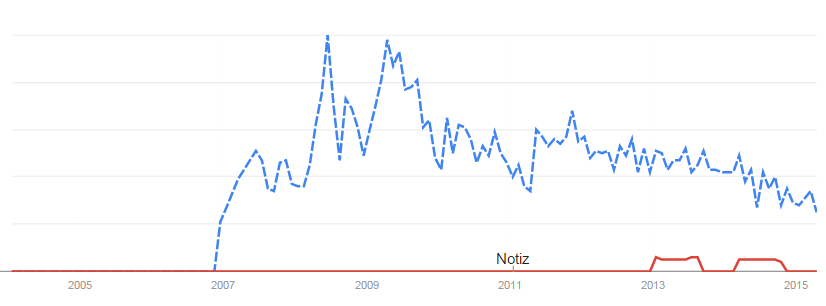
\includegraphics[width=\textwidth]{img/interesse_de.png}
\caption {Zeitverlauf des Interesses an ADF und Grails in Deutschland (Quelle: Google Trends)}
\end{figure}